\documentclass[11pt,twocolumn]{article}
\usepackage[margin=0.75in,columnsep=0.22in,top=0.6in,bottom=0.65in]{geometry}
\usepackage{graphicx,booktabs,amsmath,times,hyperref,caption}
\captionsetup{font=footnotesize,skip=2pt}
\setlength{\parskip}{0pt}\setlength{\parindent}{9pt}
\begin{document}\linespread{1.05}\selectfont
\title{\vspace{-0.4in}\large\bfseries A Vision-Based Mobile Companion Robot in MuJoCo with MediaPipe Fall Kinematics: Dispatch Latency Against Fixed Cameras\vspace{-0.1in}}
\author{\small Kamakshi Bahuguna (E007), Devanshi Sachin Kambli (B029)\\\small B.Tech CSBS, NMIMS MPSTME, MDRIIA Group 02}
\date{}
\maketitle\vspace{-0.3in}
\begin{abstract}
We study how a mobile companion robot can use MediaPipe pose kinematics to reduce emergency dispatch latency for older adults living alone. In MuJoCo, the robot follows a simulated woman through a one-bedroom flat, detects falls from bounding-box aspect ratio, hip-descent speed and torso angle, checks in by voice, and sends a simulated alert (no real call or message is ever placed). Over 120 seeded trials (60 falls, 60 daily activities, thresholds frozen on a separate dev split) the robot detected 52/60 falls (sensitivity 0.87) and dispatched 37/43 unanswered falls with 0/77 false dispatches, against 0.02 for one fixed camera and 0.48 for four. It is slower than four cameras where they see her (median 20 s vs 3.7 s), but it covers every room with one device. All dispatches fell far inside the 6-minute window. Results are simulation results from scripted motions and an earlier compact-robot variant; the guide-specification robot was verified mechanically but not evaluated at N=120.
\end{abstract}
\section{Introduction}
Surviving a cardiac arrest depends on minutes: resuscitation guidelines stress immediate CPR and defibrillation \cite{aha}, and each minute of delay to bystander CPR lowers survival for witnessed arrests \cite{nguyen}. Older adults who live alone often cannot summon help after a fall, and inability to get up is associated with lasting decline \cite{tinetti}; in a small 1981 cohort, half of the people who lay on the floor for over an hour died within six months \cite{wild}. Camera fall detectors using MediaPipe exist \cite{kothari}, and but a fixed camera sees only one room. We ask: \emph{how can a vision-based mobile companion robot in MuJoCo integrate MediaPipe fall-detection kinematics to reduce emergency dispatch latency within the 6-minute cardiac arrest survival window for elderly individuals living alone?} The robot controls only its own sphere of agency: reaching the person, detecting and confirming the event, and dispatching; ambulance travel time is outside it.
\section{Related Work}
Vision-based fall detection with pose landmarks is well established, including MediaPipe-based systems with automatic alerts \cite{kothari}; these evaluate a fixed viewpoint and report detection accuracy but not how long a household needs for the alert to reach someone, and they cannot see a room without a camera. Companion-robot work focuses on interaction rather than on measured fall-response latency. Our contribution is the paired, seeded comparison of a mobile platform against fixed cameras on the same recorded motion, with latency measured from the physical floor contact, and an economics reading that is dimensionless and conservative.
\section{Reproducibility and Ethics}
Scenarios are generated from integer seeds (dev: 1, test: 2) and every trial is replayed for all three systems. The code, the frozen thresholds, the per-trial result table and the telemetry summaries are in the project repository (folder results/small\_robot\_test). Every number in this paper is read from those files; nothing was typed or smoothed by hand. No human participants or real recordings were used, and the human model is a licensed digital character (attribution recorded in the repository). The thresholds were never tuned on the test split; two analyses that would have needed tuning (sofa suppression, follow distance) are listed as future work instead.
\section{Method}
\textbf{Simulation.} A 7$\times$6\,m flat (hall, bedroom, open living-dining area, furniture, rug ramps, a robot vacuum as a dynamic obstacle) is generated as MJCF with friction zones, joint limits and actuators. A differential-drive robot with a pan-tilt camera runs a 50\,Hz closed loop with disturbance injection (pushes, odometry noise, camera blackout) and state estimation (wheel odometry plus range-scan matching against the map). The woman is a skinned model driven by recorded gait and physics-based falls (trip, slip, syncope, cardiac) and keyframed activities of daily living (ADL): abrupt and slow sofa sitting, lying on the bed, tying shoelaces, dropping keys, sitting and lying on the floor.\\
\textbf{Perception and detection.} Frames are rendered from the robot camera and passed to the MediaPipe pose landmarker; OpenCV gives the bounding box. A fall is flagged from aspect ratio ($\ge$0.8--1.0) and its rise rate, filtered hip descent, torso pitch, then a quiet window; a still, low, horizontal person is flagged by a second path. Inference runs on the robot; frames are discarded and 0 bytes leave the robot before the first alert.\\
\textbf{Behaviour.} FOLLOW, SEARCH, OBSERVE, APPROACH (standoff 0.8--1.2\,m), CHECK\_IN (voice prompt, 10\,s), ALERT (simulated family message and ambulance call). Speed never exceeds 0.80\,m/s; emergency braking exceeds 1.5\,m/s$^2$ (2.43--3.30 measured at 0.50 and 0.79\,m/s, $\mu$ 0.40 and 0.68, pitch $\le$0.1$^\circ$).\\
\textbf{Design.} Every trial replays the same motion for the robot, one fixed camera and four fixed cameras (paired). Dev split: 40 trials, seed 1, thresholds fitted. Test split: 120 trials, seed 2, thresholds frozen. Randomised: route, speed, fall point (stratified by zone), friction, clutter, vacuum speed, push, blackout, robot start, whether she answers.
\textbf{Detector equations.} With hip height $z_h(t)$ (mean of landmarks 23 and 24), a low-pass filtered descent speed $v_z=-\dot z_h$, torso pitch $\theta$ from the shoulder--hip axis to vertical, and the landmark bounding box of width $w$ and height $h$, aspect ratio $A=w/h$ with rise rate $\dot A$, an impact is declared when $v_z$ exceeds its threshold, $\theta\ge\theta_{min}$, $A\ge A_{min}$ (or $\dot A\ge 1.0$\,s$^{-1}$) and $z_h<z_{down}$; a 3\,s quiet window must follow. Frozen robot thresholds were $z_{down}=0.45$\,m and $\theta_{min}=40^\circ$, fitted by grid search on dev replay only; the quiet (3\,s) and lying (5\,s) windows were deliberately not searched.\\
\textbf{State estimation and safety.} Odometry from the wheel encoders carries multiplicative noise (0.5--3\%); a 72-ray range scan is matched against the map every 0.25\,s, with a wide search and a whole-map search after bumps. Known walls and furniture trigger braking at 7\,cm, unknown objects (her body, the vacuum) at 25\,cm. Yaw rate is slew-limited and capped while driving to avoid wheel slip. The last metre to the standoff is controlled by the range sensor, not the landmark distance, because landmark depth proved unreliable near furniture.\\
\textbf{Telemetry.} Each trial logs time, position and orientation (x, y, z, roll, pitch, yaw), velocities ($v_x,v_y,v_z$, forward speed, yaw rate), contact forces (non-human and human separately), commanded and wheel control signals, estimated pose, detector features and bytes sent off-board, as CSV in the repository.
\begin{figure}[t]\centering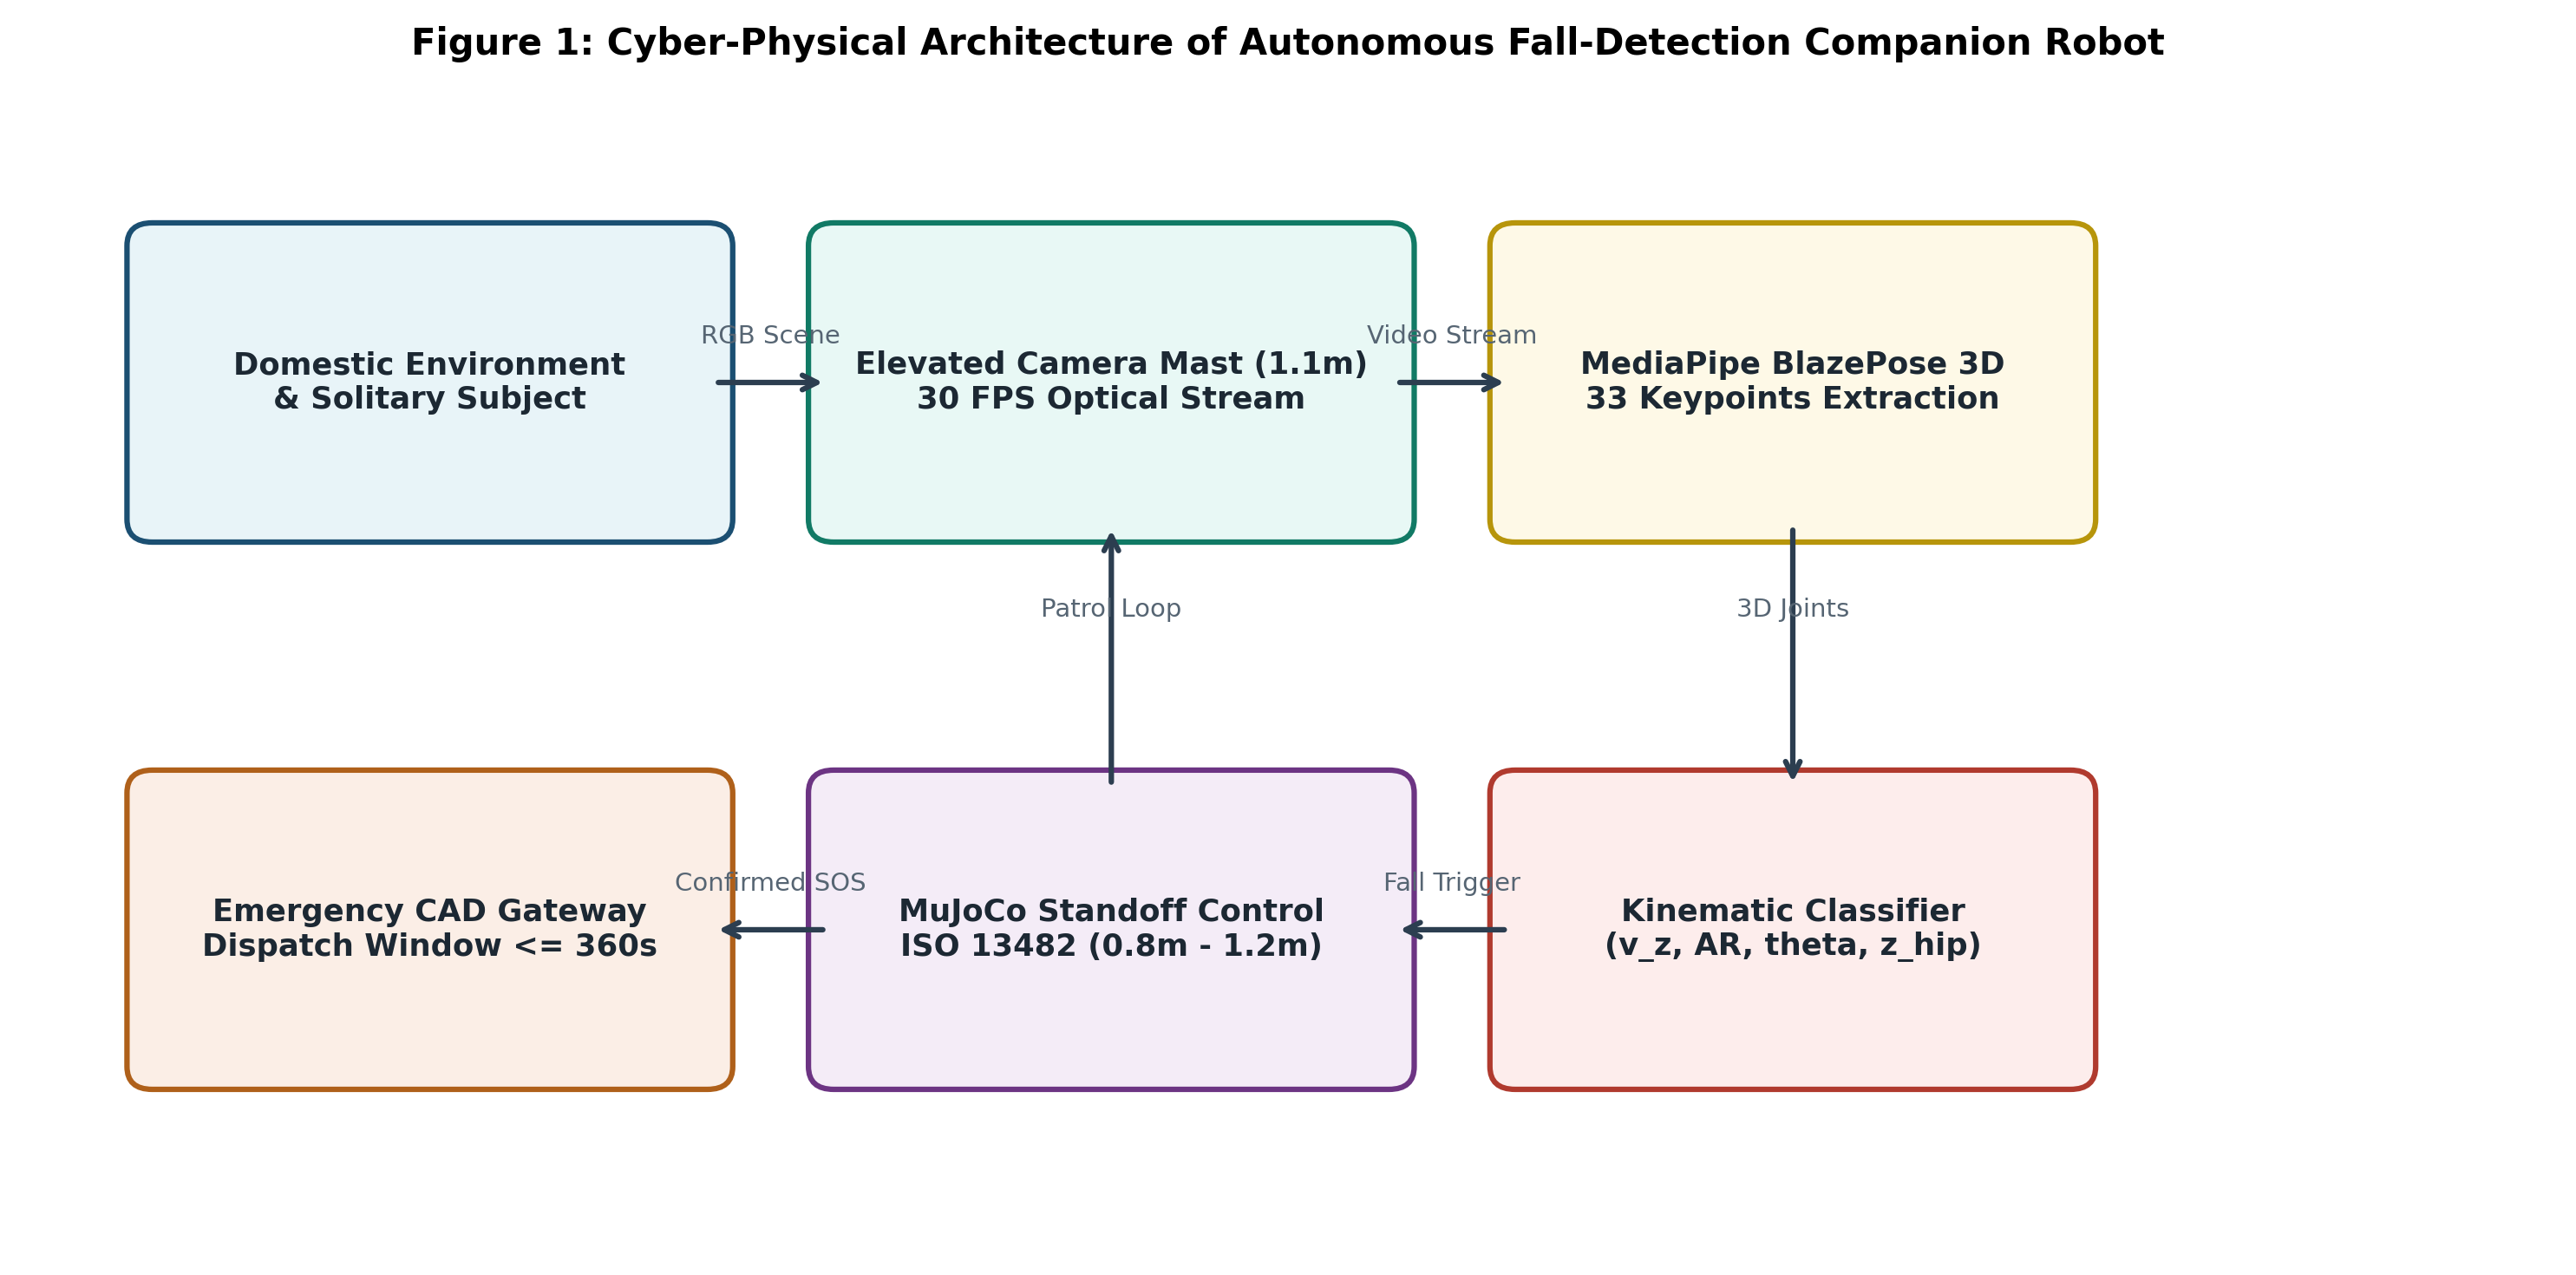
\includegraphics[width=\columnwidth]{figure1_system_architecture.png}\caption{System pipeline (drawn from the implemented modules).}\end{figure}
\section{Results}
\begin{table}[t]\centering\caption{Detection, test split (N=120). Alarm level: heads-up sent; dispatch level: emergency sent. 95\% Wilson CI in brackets.}\footnotesize
\begin{tabular}{@{}llccc@{}}\toprule Level & System & Sensitivity & Specificity & F1\\\midrule
Alarm & Robot & 0.87 [.76,.93] & 0.75 [.63,.84] & 0.82\\
Alarm & 4 cameras & 0.48 [.36,.61] & 0.98 [.91,1.0] & 0.64\\
Alarm & 1 camera & 0.02 [.00,.09] & 1.00 & 0.03\\
Dispatch & Robot & 0.86 [.73,.93] & 1.00 [.95,1.0] & 0.93\\
Dispatch & 4 cameras & 0.47 [.33,.61] & 1.00 & 0.64\\
Dispatch & 1 camera & 0.02 [.00,.12] & 1.00 & 0.05\\\bottomrule\end{tabular}\end{table}
The robot flagged 52/60 falls and dispatched 37/43 unanswered falls (precision 1.00, recall 0.86), with no false dispatch in 77 non-events. At alarm level specificity is 0.75: all 10 deliberate floor activities and 5/20 sofa sits raised a heads-up text, and the check-in answer cleared every one before dispatch. Sofa false alarms coincide with landmark estimates collapsing behind the sofa (hypothesis, not isolated). McNemar tests: robot-only detections 28 vs 5 for four cameras ($p=7\times10^{-5}$) and 51 vs 0 for one camera ($p<10^{-15}$).
\begin{figure}[t]\centering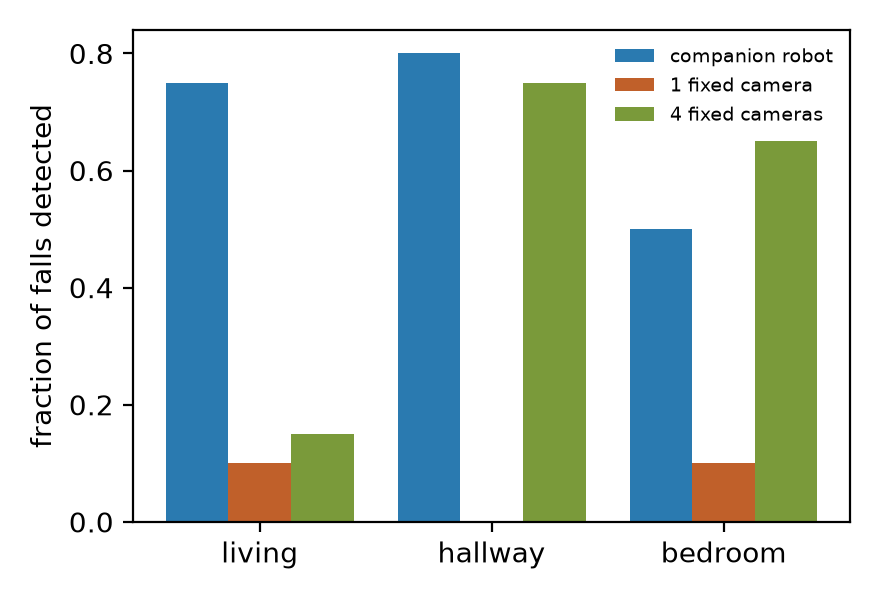
\includegraphics[width=\columnwidth]{detection_by_zone.png}\caption{Falls detected by where she fell (n=20 per zone). The four cameras see nothing in the living area; the robot covers all zones.}\end{figure}
\begin{table}[t]\centering\caption{Latency from hip floor contact (s), successful detections only; SE = standard error.}\footnotesize
\begin{tabular}{@{}llrrrr@{}}\toprule Level & System & n & Mean$\pm$SE & Median & P95\\\midrule
Heads-up & Robot & 52 & 26.4$\pm$3.1 & 20.3 & 67.1\\
Heads-up & 4 cameras & 28 & 4.3$\pm$0.3 & 3.7 & 5.3\\
Dispatch & Robot & 37 & 42.5$\pm$3.8 & 39.8 & 82.4\\
Dispatch & 4 cameras & 19 & 14.3$\pm$0.4 & 13.5 & 16.0\\\bottomrule\end{tabular}\end{table}
Where both detected (paired), the robot was slower by 30.1\,s (95\% CI 21.3--39.0, $t(23)=7.03$, $p=3.7\times10^{-7}$, Cohen's $d=1.43$). Within 60\,s the robot dispatched 65\% of silent falls (four cameras 44\%, one camera 2\%); within 100\,s, 86\%. Every dispatch occurred inside 90\,s, far under the 360\,s window.
\begin{figure}[t]\centering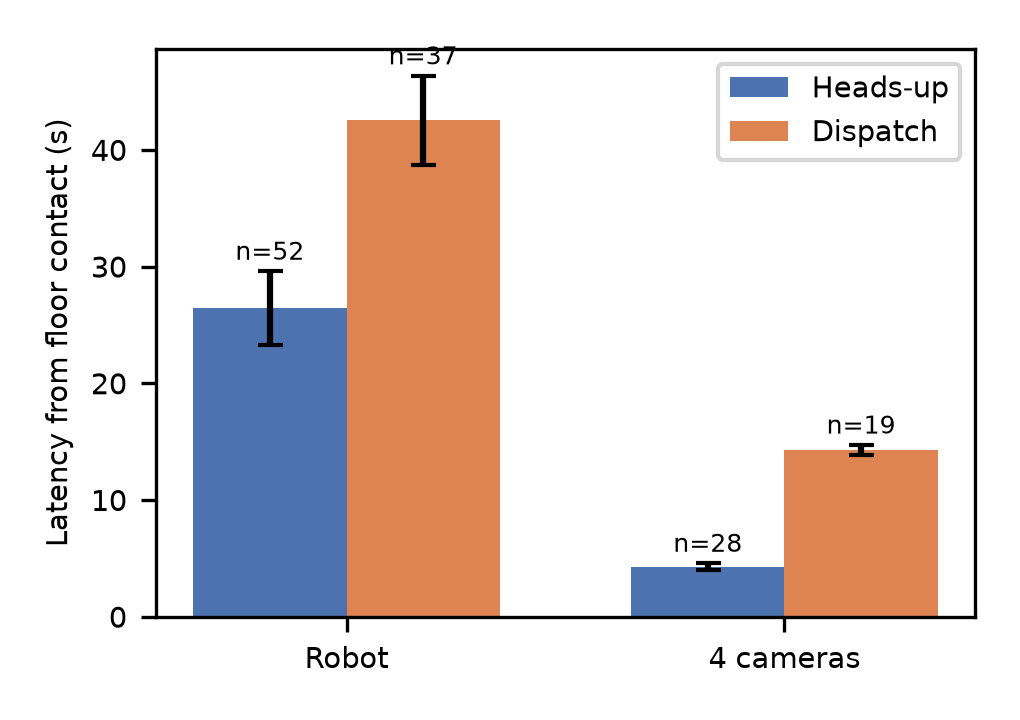
\includegraphics[width=0.9\columnwidth]{latency_se.png}\caption{Mean latency $\pm$ SE.}\end{figure}
\textbf{Economics (dimensionless).} With a long-lie reduction from 18.4 to 4.2 hospital days (sheet value) applied to detected falls, the robot yields 14.7 net bed-days per patient-year versus 7.9 for four cameras and 0.4 for one camera. With operating fraction $\kappa=0.20$ ($\le0.25$) and a capital cost of the brief's upper bound (3 attendant-months), payback is $12K_0/(1-\kappa)=3.75$ months, longer than one quarter. The brief's two claims (cost under 3 months of attendant cost, return within one quarter) agree only if the capital cost is at most $3(1-\kappa)$ months, i.e.\ 2.4 months at $\kappa=0.20$ (payback exactly 3.0); we report 3.75 months for the bound and leave the cost ratio as an assumption. Zero false dispatches in 77 negatives bounds the false-dispatch rate only below 4.8\% (95\%), while $\kappa$ needs $\le0.51\%$: about 585 negative trials would be needed. GDS peace of mind cannot be simulated.
\section{Discussion}
\textbf{Coverage versus speed.} The fixed cameras detect within 3--5\,s because they watch continuously and need no travel. The robot pays for travel and search: its heads-up latency is 2.9--75\,s and depends on where she falls (median 5.6\,s in the living area, 36\,s in the hall, 52\,s in the bedroom). Against one camera, the only comparison at equal hardware cost, the robot wins decisively; against four cameras it detects more falls (52 vs 29) but later. A household would buy the robot for rooms a camera cannot cover, not for speed in the room where a camera already looks.\\
\textbf{Where it fails.} Missed falls (8/60) are coverage or search failures, not threshold failures: nobody saw her. Eight trials ended with localisation lost, mostly while searching the west living room and bedroom. One cardiac collapse landed on the robot because it followed too close in the landing zone; a future version should follow from the side and farther back when she looks unwell. The false alarms on sofa sitting raise the exact pitfall the brief names; a map-based suppression (hip above a mapped seat) is the obvious next step and would need a new seed to evaluate.\\
\textbf{Privacy.} Processing is on-board, frames are discarded, and 0 bytes left the robot before the first alert (maximum over all trials). After an alert, at most one face-blurred snapshot is sent, and only if she consented.\\
\textbf{Honest scope.} A camera cannot diagnose a heart attack. The robot detects a collapse, no movement and no reply, and its alert says ``possible medical emergency''. All calls and messages are simulated payloads. The hospital-stay reduction (18.4 to 4.2 days), the 134.5-minute ambulance figure and the 6-minute window are taken from the course brief; we could not trace the first two to a primary source and the 1981 mortality figure rests on 20 people, so they are stated as assumptions, not as findings. The ``50\% mortality attributed to Tinetti, NEJM'' in the brief is not in that paper (JAMA 1993); the half-died-within-six-months result is from the 1981 BMJ cohort.
\section{Limitations}
(i) The 120-trial test ran on an earlier compact-robot variant with a 0.16\,m camera; the guide-specification robot (1.10\,m mast, 16.5\,kg, tip limit 7.76 vs guide 7.64\,m/s$^2$) was verified mechanically and its dev run was unsatisfactory (contacts and lost localisation), so its test was not completed. (ii) Motions are scripted from clinical descriptions, adult body, not patient data; cardiac prodrome cues false-flagged 49\% of non-cardiac trials and are not used for alerting. (iii) 8/120 robot trials ended lost (pose error $>0.5$\,m); one cardiac fall landed on the robot (4580\,N); max non-human contact 12\,N. (iv) The robot is slower than four cameras where they see; the claim is coverage, not speed. (v) The 0.50\,m clearance bubble cannot be kept in 0.85\,m doors, so it is a speed rule. (vi) The fixed-camera baseline is hardware-limited; thresholds were fitted on dev replay.
\section{Conclusion}
A mobile robot buys coverage: with one device it detected 87\% of simulated falls across all rooms and dispatched within 100\,s in 86\% of silent falls, where one camera saw 2\% and four cameras 48\%. It does not beat four cameras on speed. Medication reminders, the Momo agent, the family platform and the siren are demo extras outside these measurements. Code, seeds and result tables are in the project repository.
\begin{thebibliography}{9}\footnotesize
\bibitem{nguyen}H.~Nguyen \emph{et al.}, ``Association between delays in time to bystander CPR and survival for witnessed cardiac arrest,'' \emph{Circ. Cardiovasc. Qual. Outcomes}, 2024, doi:10.1161/CIRCOUTCOMES.123.010116.
\bibitem{tinetti}M.~E. Tinetti, W.-L. Liu, E.~B. Claus, ``Predictors and prognosis of inability to get up after falls among elderly persons,'' \emph{JAMA}, vol.~269, no.~1, pp.~65--69, 1993, doi:10.1001/jama.1993.03500010075035.
\bibitem{wild}D.~Wild, U.~S. Nayak, B.~Isaacs, ``How dangerous are falls in old people at home?'' \emph{Br. Med. J.}, vol.~282, no.~6260, pp.~266--268, 1981, doi:10.1136/bmj.282.6260.266.
\bibitem{kothari}Kothari \emph{et al.}, ``Towards safer environments: a YOLO and MediaPipe-based human fall detection system with alert automation,'' \emph{MethodsX}, 2025, doi:10.1016/j.mex.2025.103623.
\bibitem{aha}M.~R. Panchal \emph{et al.}, ``Part 3: Adult basic and advanced life support: 2020 AHA guidelines for CPR and emergency cardiovascular care,'' \emph{Circulation}, 2020, doi:10.1161/CIR.0000000000000916.
\end{thebibliography}
\end{document}
